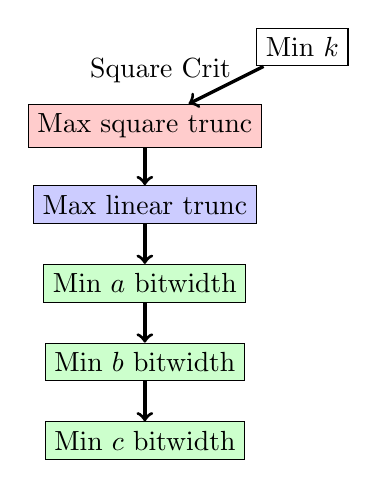
\begin{tikzpicture}

\node [shape=rectangle,draw = black, minimum width = 1cm] at (2,3) (min_k_lut_crit) {Min $k$};

% Square Crit DSE Method
\node at (0.2,2.7) {Square Crit};
\node [shape=rectangle,draw = black, minimum width = 1cm, fill=red!20]   at (0,2) (sq_trunc_sq_crit) {Max square trunc};
\node [shape=rectangle,draw = black, minimum width = 1cm, fill=blue!20]  at (0,1) (lin_trunc_sq_crit) {Max linear trunc};
\node [shape=rectangle,draw = black, minimum width = 1cm, fill=green!20] at (0,0) (a_prec) {Min $a$ bitwidth};
\node [shape=rectangle,draw = black, minimum width = 1cm, fill=green!20] at (0,-1) (b_prec) {Min $b$ bitwidth};
\node [shape=rectangle,draw = black, minimum width = 1cm, fill=green!20] at (0,-2) (c_prec) {Min $c$ bitwidth};

\draw [->,very thick] (min_k_lut_crit) edge (sq_trunc_sq_crit);
\draw [->,very thick] (sq_trunc_sq_crit) edge (lin_trunc_sq_crit);
\draw [->,very thick] (lin_trunc_sq_crit) edge (a_prec);
\draw [->,very thick] (a_prec) edge (b_prec);
\draw [->,very thick] (b_prec) edge (c_prec);

% LUT Crit DSE Method
% \node at (3.8,2.7) {LUT Crit};
% \node [shape=rectangle,draw = black, minimum width = 1cm, fill=green!20] at (4,2) (lut_width) {Min LUT width};
% \node [shape=rectangle,draw = black, minimum width = 1cm, fill=red!20]   at (4,1) (sq_trunc_lut_crit) {Max square trunc};
% \node [shape=rectangle,draw = black, minimum width = 1cm, fill=blue!20]  at (4,0) (lin_trunc_lut_crit) {Max linear trunc};

% \draw [->,very thick] (min_k_lut_crit) edge (lut_width);
% \draw [->,very thick] (lut_width) edge (sq_trunc_lut_crit);
% \draw [->,very thick] (sq_trunc_lut_crit) edge (lin_trunc_lut_crit);


\end{tikzpicture}